\chapter{triangular\_shelf}

\section{Purpose}

To compare TELEMAC-2D simulation with a benchmark
(\url{http://isec.nacse.org/workshop/2009_isec/benchmarks.html#bmark1}).

\section{Description}

\subsection{Geometry and mesh}

Size of the model: rectangle (48.8m x 26.5m)
Water Depth: 0.78 m

The Figure~\ref{fig:triang:geometry} shows the geometry of the study.
\begin{figure}
\centering
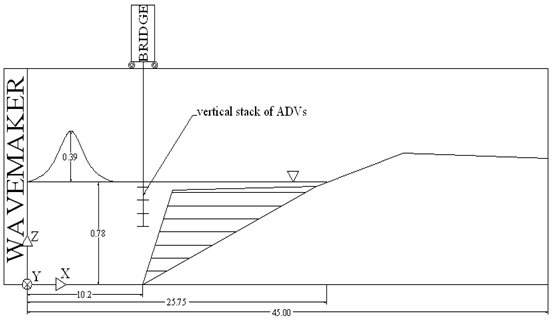
\includegraphics[width=.6\textwidth]{img/geom.png}
\caption{Geometry of the study}\label{fig:triang:geometry}
\end{figure}

\begin{itemize}
  \item Nodes: 18720
  \item Elements: 36874
\end{itemize}

The Figure~\ref{fig:triang:mesh} shows the mesh of the study.
\begin{figure}
\centering
\includegraphics[width=.6\textwidth]{../img/Mesh.png}
\caption{Mesh of the study}\label{fig:triang:mesh}
\end{figure}


The Figure~\ref{fig:triang:bathy} shows the bathymetrie of the study.
\begin{figure}
\centering
\includegraphics[width=.6\textwidth]{../img/Bathy.png}
\caption{Bathymetrie of the study}\label{fig:triang:bathy}
\end{figure}


\subsection{Boundaries}

The Figure~\ref{fig:triang:boundaries} shows the boundaries of the study.
\begin{figure}
\centering
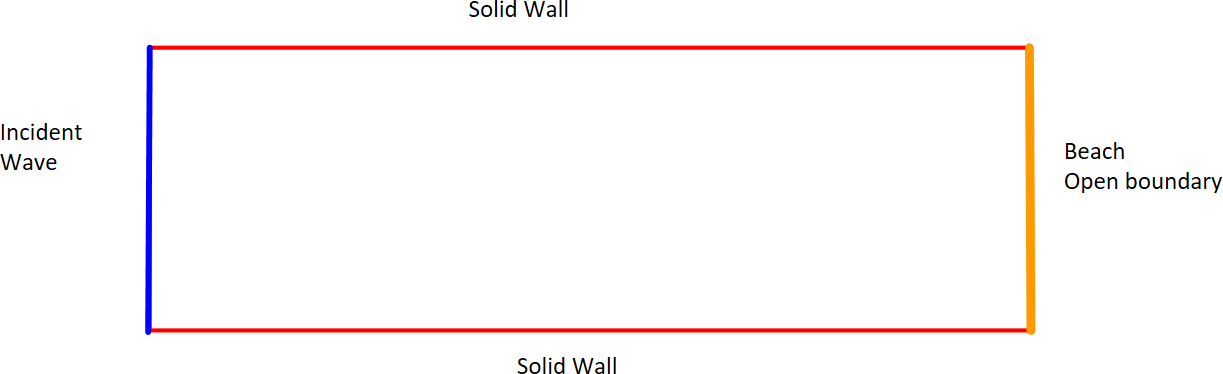
\includegraphics[width=.6\textwidth]{img/boundaries.png}
\caption{Geometry of the study}\label{fig:triang:boundaries}
\end{figure}

Single solitary wave generated (H = 0.39 m)

Bottom:
\begin{itemize}
  \item Chezy's Law
  \item Friction coefficient: 180
\end{itemize}

\subsection{Physical parameters}

Turbulence: Constant viscosity equal to zero

\section{Numerical parameters}

\begin{itemize}
  \item Type of element: P1 triangle for h and for velocity
  \item Solver: GMRES
  \item Accuracy: $10^{-6}$
  \item Finite volume scheme: Kinetic order 2
\end{itemize}

\begin{table}[H]
  \begin{center}

    \begin{tabular*}{.9\textwidth}{|c|c|c|}
  \hline
  Equations & Saint-Venant VF & Boussinesq \\
  Time step & 0.05 & 0.005 \\
  Simulation duration & 45 & 45 \\
  \hline
\end{tabular*}
  \end{center}
\end{table}

\section{Results}
We compare the model and experiment free surface at
\begin{itemize}
  \item X = 25 m
  \item Y =  0 m
  \item Y = -5 m
\end{itemize}

The Figure~\ref{fig:triang:vel} shows the velocity vectors.
\begin{figure}
\centering
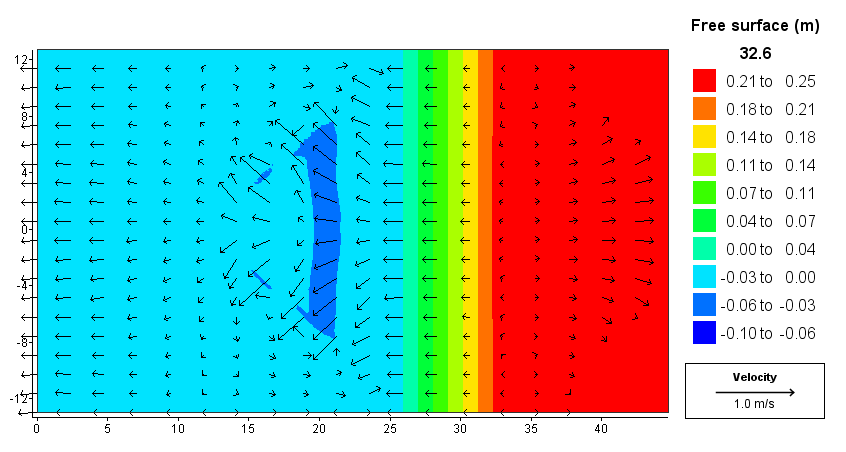
\includegraphics[width=.6\textwidth]{img/vel.png}
\caption{Velocity vectors over the free surface}\label{fig:triang:vel}
\end{figure}

The Figure~\ref{fig:triang:res} shows the comparison with the benchmark data.
\begin{figure}
\centering
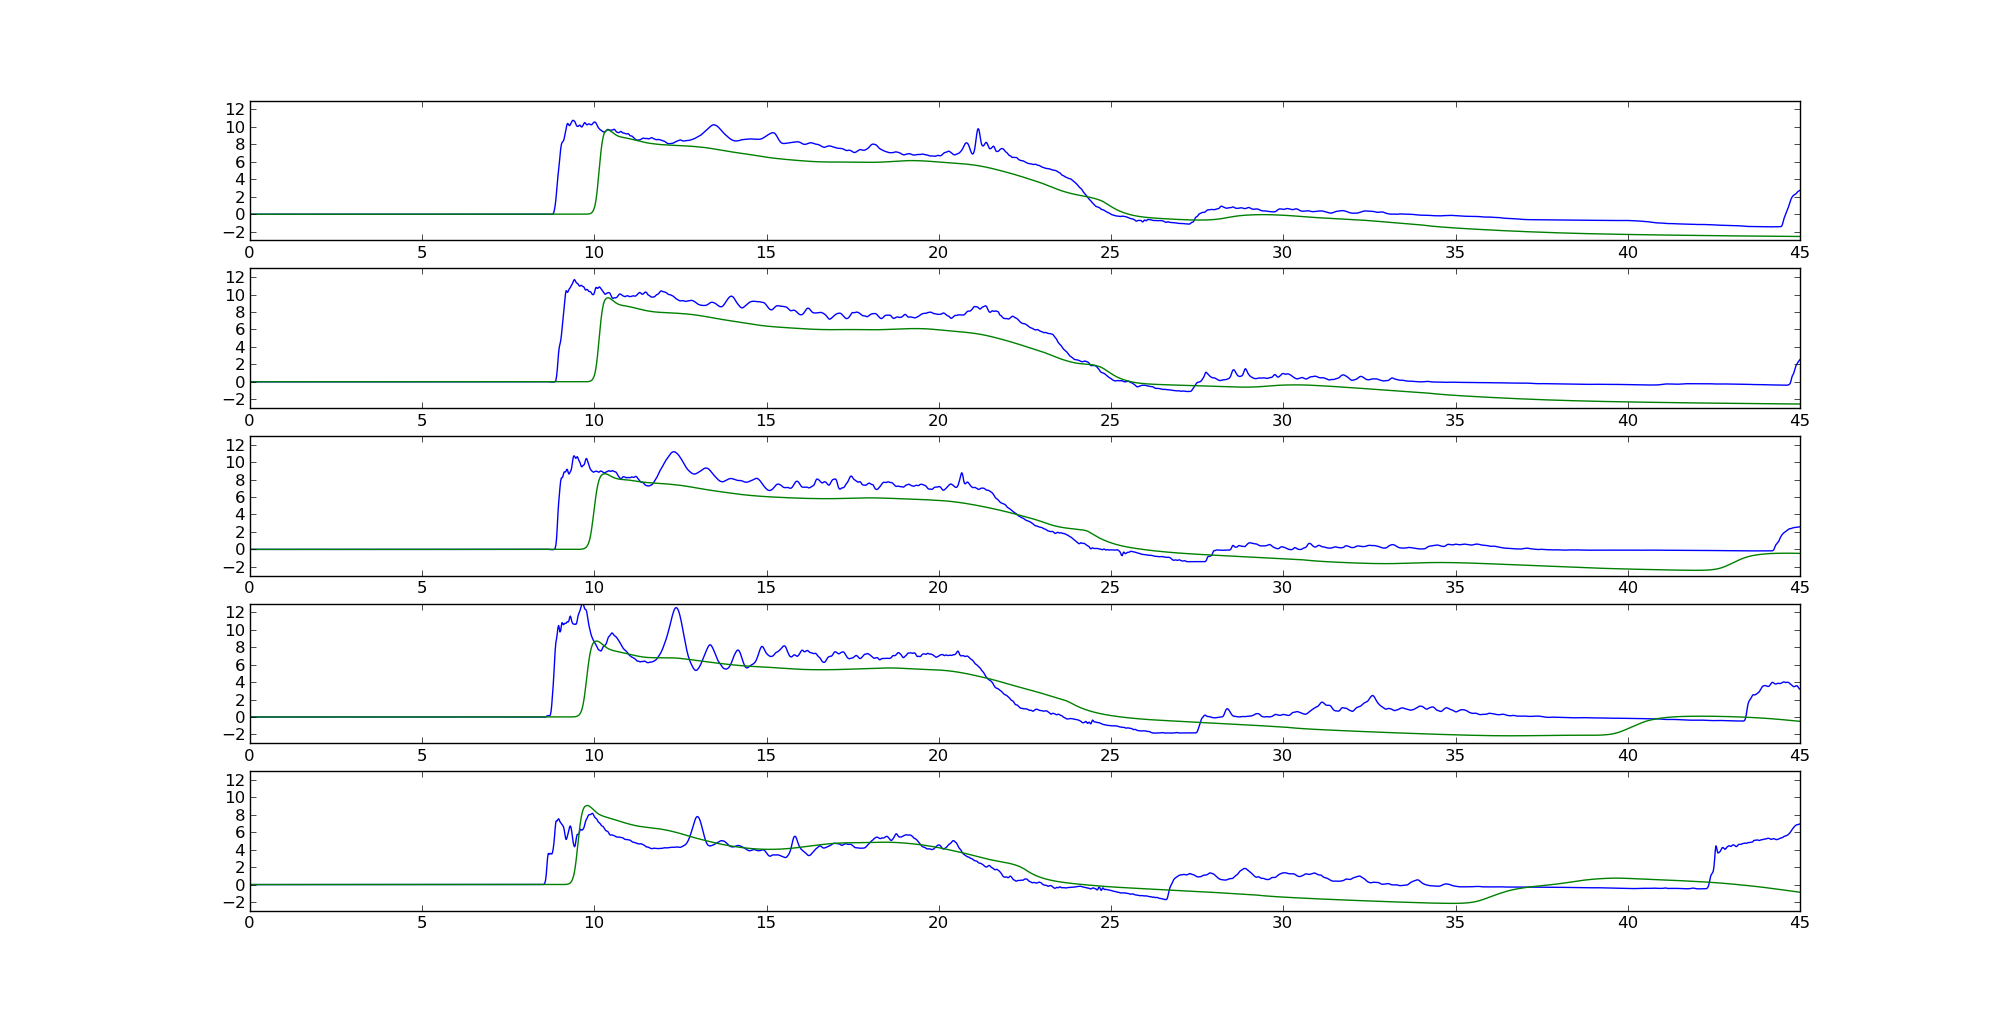
\includegraphics[width=.8\textwidth]{img/res_X25.png}
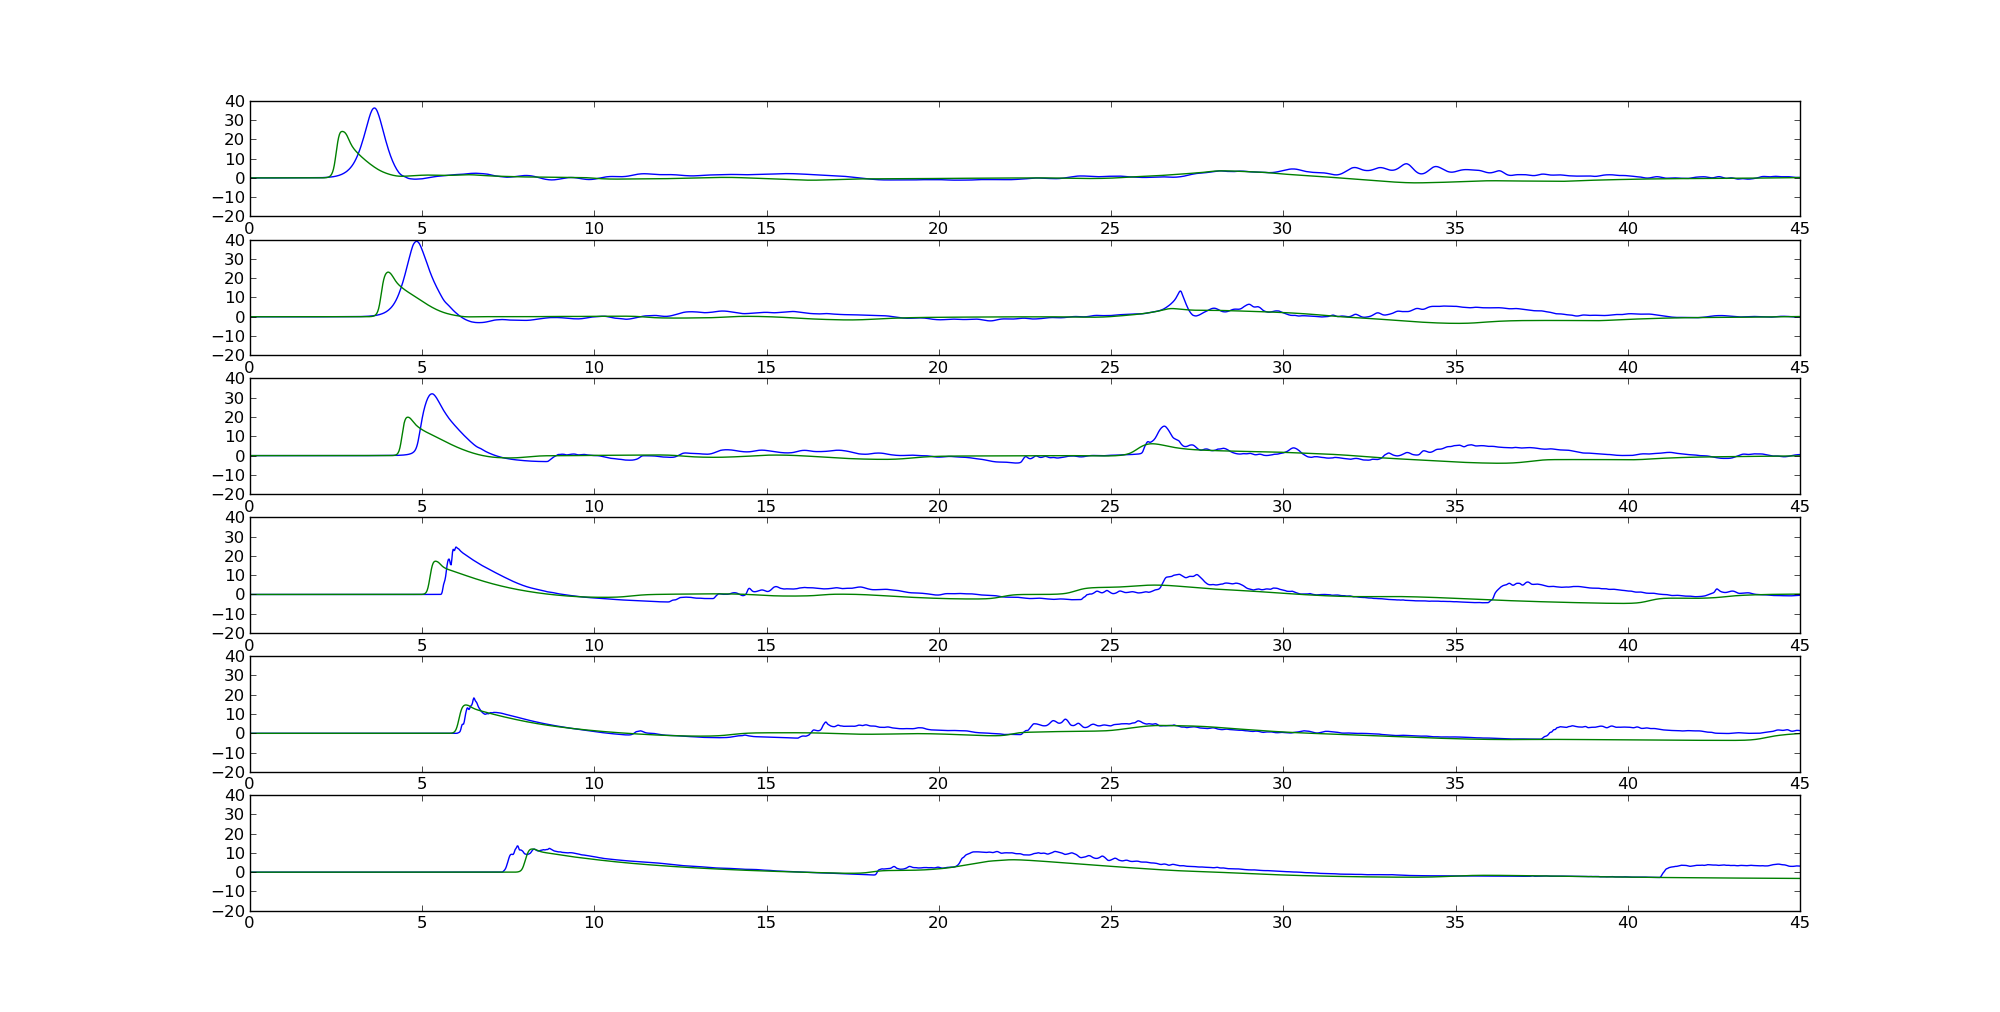
\includegraphics[width=.8\textwidth]{img/res_Y0.png}
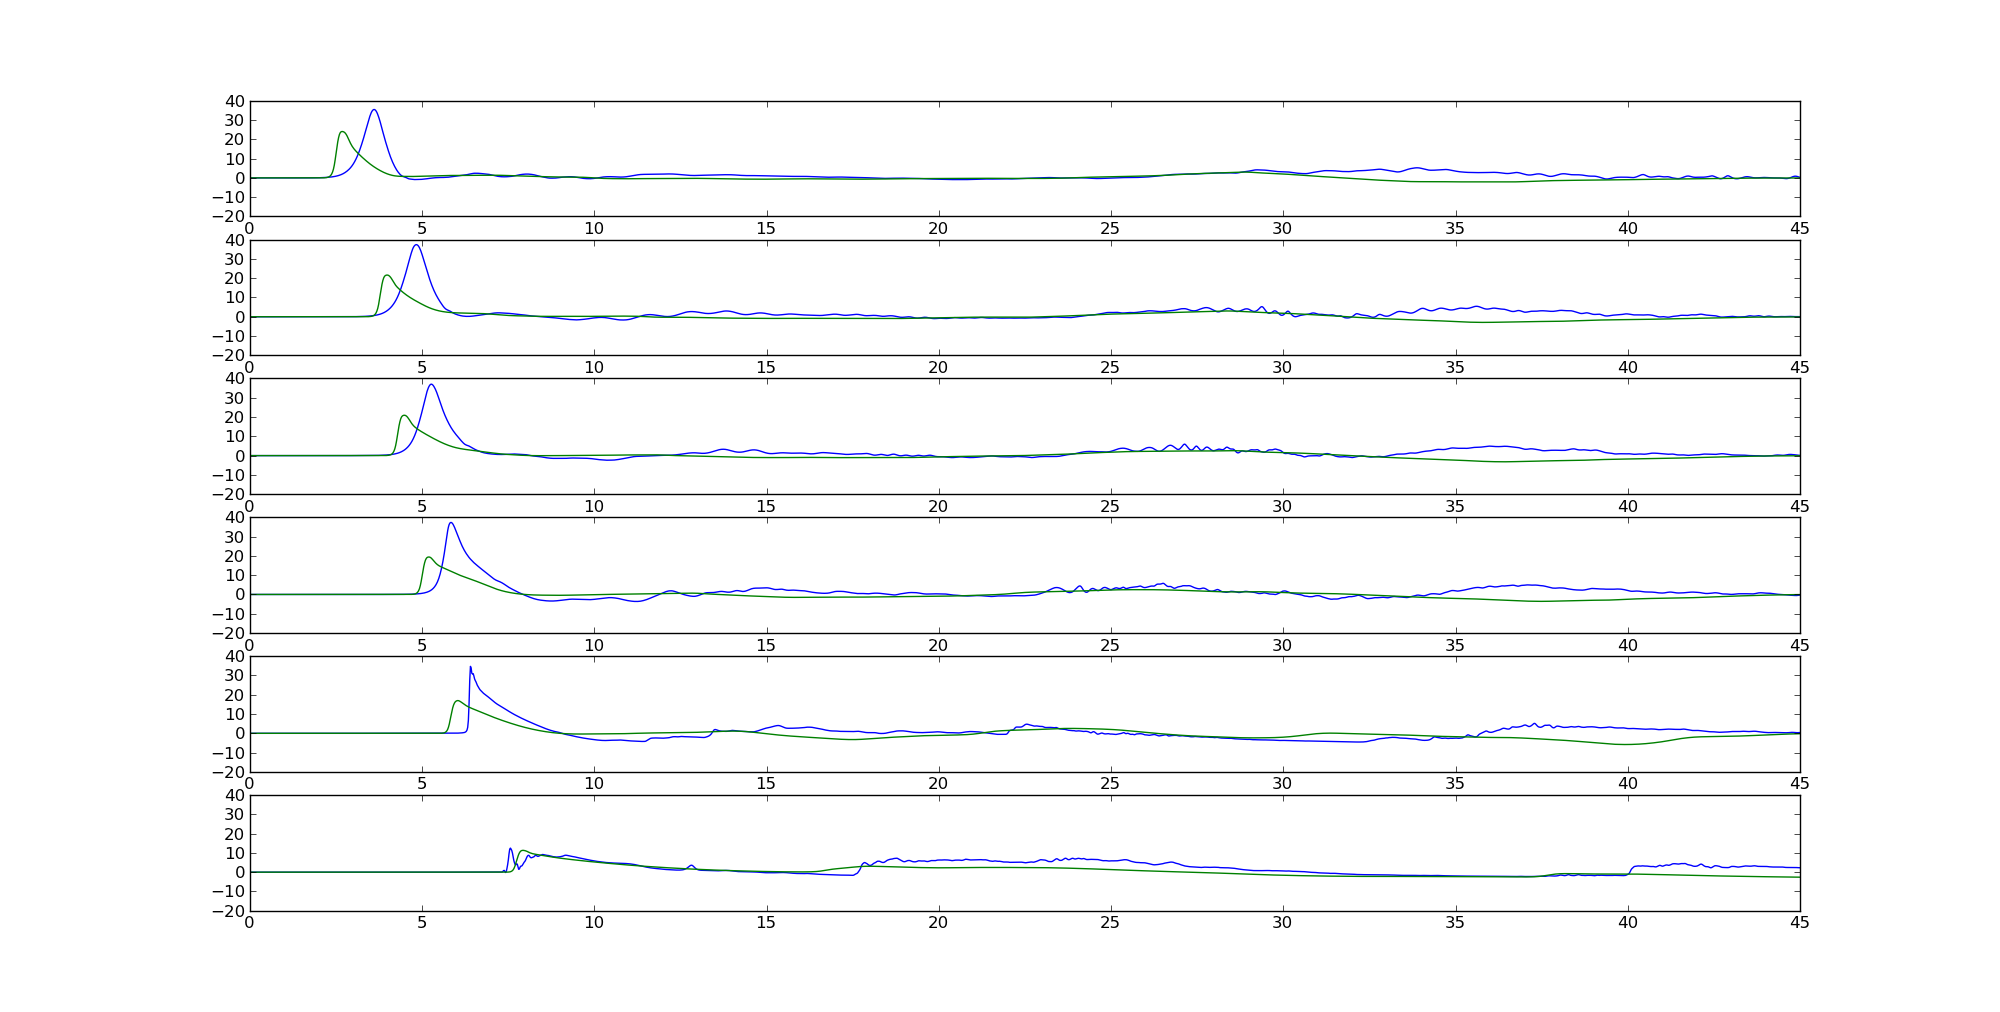
\includegraphics[width=.8\textwidth]{img/res_Y-5.png}
\caption{Comparaison of the results If blue the expermient and in green the model}\label{fig:triang:res}
\end{figure}
